\documentclass[twocolumn,a4paper,10pt]{article}

\usepackage[utf8]{inputenc}
\usepackage{t1enc}
\usepackage[spanish]{babel}
\usepackage[pdftex,usenames,dvipsnames]{color}
\usepackage[pdftex]{graphicx}
\usepackage{enumerate}
\usepackage{url}
\usepackage{amsmath}
\usepackage{amsfonts}
\usepackage{amssymb}
\usepackage[table]{xcolor}
\usepackage[small,bf]{caption}
\usepackage{float}
\usepackage{subfig}
\usepackage{bm}
\usepackage{fancyhdr}
\usepackage{times}
\usepackage{titlesec}
\usepackage[numbers]{natbib}
\usepackage{titling}
\usepackage{listings}

\renewcommand{\lstlistingname}{Código Fuente}

%%% Listings
\lstloadlanguages{Octave} 
\lstdefinelanguage{MyOctave}[]{Octave}{% 
	deletekeywords={beta,det},
	morekeywords={repmat}
} 
\lstset{ %
	language=MyOctave,
	stringstyle=\ttfamily,
	showstringspaces = false,
	basicstyle=\footnotesize\ttfamily,
	commentstyle=\color{gray},
	keywordstyle=\bfseries,
	numbers=left,
	numberstyle=\ttfamily\footnotesize,
	stepnumber=1,                   % the step between two line-numbers. If it's 1 each line will be numbered
	framexleftmargin=0.10cm,
	numbersep=0.05cm,               % how far the line-numbers are from the code
	backgroundcolor=\color{white},
	showspaces=false,
	showtabs=false,
% 	frame=l,
	tabsize=4,
	captionpos=b,                   % sets the caption-position to bottom
	breaklines=true,                % sets automatic line breaking
	breakatwhitespace=false,        % sets if automatic breaks should only happen at whitespace
	mathescape=true
}

\def\customabstract{\vspace{.5em}
    {\small\center{\textbf{RESUMEN}} \\[0.5em] \relax%
}}
\def\endkeywords{\par}

\def\keywords{\vspace{.5em}
    {\textit{Palabras clave: } 
}}
\def\endkeywords{\par}

\titleformat{\section}{\small\center\bfseries}{\thesection.}{0.5em}{\normalsize\uppercase}
\titleformat{\subsection}{\small\center\bfseries}{\thesubsection}{0.5em}{\small\uppercase}
\titleformat{\subsubsection}{\small\bfseries}{}{0.5em}{\small}
\renewcommand{\bibsection}{}

% TITLE Configuration
\setlength{\droptitle}{-30pt}
\pretitle{\begin{center}\Huge\begin{rmfamily}}
\posttitle{\par\end{rmfamily}\end{center}\vskip 0.5em}
\preauthor{\begin{center}
        \large \lineskip 0.5em%
\begin{tabular}[t]{c}}
\postauthor{\end{tabular}\normalsize 
    \\[1em] Estudiantes del Instituto Tecnológico de Buenos Aires
\par\end{center}}
\predate{\begin{center}\small}
\postdate{\par\end{center}}

% Headers
\addtolength{\voffset}{-40pt}
\addtolength{\textheight}{80pt}
\renewcommand{\headrulewidth}{0pt}
\fancyhead{}
\fancyfoot{}
\lhead{\small No publicado: Cátedra de Métodos Numéricos Avanzados (ITBA)}
\rhead{\small \thepage}
\cfoot{\small Copyright \copyright 2012 ITBA}

% Metadata
\title{Procesamiento de Imagenes}
\date{23 de Noviembre de 2012}
\author{Civile, Juan Pablo \and Crespo, Álvaro \and Ordano, Esteban }

\begin{document}

\pagestyle{fancy}
\maketitle
\thispagestyle{fancy}

\begin{customabstract}
\textbf{
El objetivo del presente trabajo es realizar un an\'alisis espectral de una imagen y utilizar la Transformada Discreta de Fourier en 2 dimensiones para 
la aplicaci\'on de filtros en el dominio de frecuencias, también conocidos como espaciales.
}
\end{customabstract}

\begin{keywords}
Transformada Discreta de Fourier en 2 dimensiones, Filtros espaciales, Fast Fourier Transform, an\'alisis espectral, dominio espacial, dominio de frecuencias
\end{keywords}

\section{Introducci\'on}

La Transformada de Fourier es una herramienta muy importante para el procesamiento de im\'agenes, la cual se usa para descomponer una imagen en sus 
componenetes de senos y cosenos. La salidad de la transformaci\'on representa la imagen en el dominio de frecuencia o dominio de Fourier, mientras 
que la entrada es el dominio espacial equivalente. En la imagen del dominio de frecuencias, cada punto representa una frecuencia particular contenida en el 
dominio espacial de la imagen. \\

La Transformada de Fourier se utiliza para una gran variedad de aplicaciones, como ser an\'alisis, filtrado, compresi\'on y reconstrucci\'on de im\'agenes. \\

Una imagen en escala de grises, como la que se desea estudiar, puede pensarse como una funci\'on en 2 dimensiones $f(x,y)$ donde el valor de la función
para cada $x,y$ está dado por la intensidad luz en esa posici\'on. Dicha intensidad se mide de 0 (ausencia de luz, color negro) a 255 (m\'axima intensidad, 
color blanco). En el presente trabajo, se utilizará esta concepci\'on para la aplicaci\'on de filtros espaciales, via la 
Transformada Discreta de Fourier en 2 dimensiones. \\

La Transformada Discreta de Fourier en 2 dimensiones, así como la Transformada Inversa Discreta, se encuentran definidas en la secci\'on 
\ref{sec:defDFT}.\\
En la secci\'on \ref{sec:metodologia} se explica la metodolog\'ia usada para la obtenci\'on de las im\'agenes correspondientes a la amplitud 
y a la fase, y para aplicaci\'on de los filtros. \\
En la secci\'on \ref{sec:resultados} se muestran los resultados obtenidos, junto con el an\'alisis de cada uno. \\
Finalmente, en la secci\'on \ref{sec:conclusiones} se resumen los conceptos y las conclusiones m\'as importantes. \\

Al final de este documento, se encuentra el Anexo, el cual contiene el c\'odigo fuente de todos los programas utilizados (Anexo 1) y 
las im\'agenes obtenidas como resultado y referenciadas a lo largo del presente trabajo (Anexo 2).\\

Todos los resultados se obtienen a partir de la Figura \ref{fig:saturno}, la cual es una imagen en escala de grises del planeta Saturno. \\

\section{Transformada Discreta de Fourier en 2 dimensiones}
\label{sec:defDFT}
La Transformada Discreta de Fourier de una secuencia bidimensional $x_{n,m}$ de $N \times N$ (en nuestro caso, la imagen) 
se define como \cite{Guia2-MNA} \cite{NumericalRecipes}:

\begin{equation}
    X_{l,k} = \sum_{n=0}^{N - 1} \sum_{m=0}^{N - 1} x_{n,m} e^{-i*\frac{2*\pi}{N}*(nl + mk)}
\end{equation}

siendo la Transformada Inversa Discreta

\begin{equation}
    x_{n,m} = \frac{1}{N^2} \sum_{l=0}^{N - 1} \sum_{k=0}^{N - 1} X_{l,k} e^{i*\frac{2*\pi}{N}*(nl + mk)}
\end{equation}

Anexadas al presente trabajo se encuentran nuestras implementaciones, tanto de la Transformada Discreta (Anexo: C\'odigo Fuente \ref{code:dft}) como de
 la Transformada Inversa Discreta (Anexo: C\'odigo Fuente \ref{code:idft}) . 
Sin embargo, es f\'acil ver que estas 
implementaciones son de orden $O(n^2)$ para calcular cada elemento de la matriz, por lo que aplicar nuestra implementaci\'on de la 
transformada (o de la transformada inversa) a una matriz ser\'ia orden $O(n^4)$. Teniendo esto en cuenta, y agregando el hecho de que nuestra imagen es de 400 $x$ 400 
pixeles, se hace necesario recurrir a una implementaci\'on m\'as eficiente. Es por esto que para la obtenci\'on de los resultados y su posterior an\'alisis 
se utilizan las funciones \textit{built-in} de \textit{Octave}, \textit{fft2} y \textit{ifft2}, que implementan algoritmos del estilo FFT 
(\textit{Fast Fourier Transform}) \cite{Wikipedia_FFT}.\\

Se encuentra anexado también para el lector el c\'odigo fuente de un sencillo programa de prueba que compara, para una matriz de un tamaño pequeño, 
los resultados obtenidos a  partir de nuestras implementaciones contra los de las funciones de \textit{Octave}
(Anexo: C\'odigo Fuente \ref{code:dft_test} y \ref{code:idft_test}). \\

\section{Metodolog\'ia}
\label{sec:metodologia}

\subsection{Imagen en amplitud y en fase. Recupero de imagen original.}

Para hallar la imagen en amplitud, se procede aplicando la Transformada Discreta de Fourier en 2 dimensiones a nuestra imagen y qued\'andonos con el 
m\'odulo. Cabe destacar que la Transformada Discreta devuelve n\'umeros complejos. El centro de la imagen de amplitud, representa las frecuencias bajas, 
mientras que las partes más cercanas a los bordes representan las frecuencias m\'as altas \cite{HIPR2-FourierTransform}.\\

Para hallar la imagen en fase, el proceso es el mismo, excepto que en lugar de quedarnos con el m\'odulo de los n\'umeros complejos, nos quedamos con el 
\'angulo o argumento. Tambi\'en se agrega una normalizaci\'on, para mapear los valores de fase al intervalo entero $[0, 255]$, 
requerido para representar la escala de grises.\\

Finalmente, se aplica la Transformada Inversa Discreta a la imagen transformada para reconstruir la imagen original.\\

\subsection{Aplicaci\'on de filtros}
\label{sec:aplicacionFiltros}

Para la aplicaci\'on de un filtro sobre la imagen se requiere que la funci\'on que act\'ua como filtro est\'e bien definida para todo elemento de la imagen.
Teniendo esto en cuenta, se obtiene la imagen transformada (imagen en frecuencias), se multiplica \textit{elemento a elemento} por el filtro deseado, y 
finalmente se aplica la Transformada Inversa Discreta para recuperar la imagen fitrada. \\

A continuaci\'on se explicitan las funciones de los filtros analizados en este documento. \\

\subsubsection{Filtro Custom}

Definimos el filtro custom a utilizar como:

\begin{equation}
    H_{k,l} = \left\{
                    \begin{array}{c l}
                        0 & \mbox{si } 0 \leq k \leq 400, 190 \leq l \leq 210\\
                        0 & \mbox{si } 0 \leq l \leq 400, 190 \leq k \leq 210\\
                        1 & \mbox{en todo otro caso}
                    \end{array}               
               \right.
\end{equation}

\subsubsection{Filtro Gaussiano}

El filtro gaussiano se define de la siguiente manera:

\begin{equation}
    H_{k,l} = exp(-0,1(k^2 + l^2))
\end{equation}


\subsubsection{Filtro Damero}

Definimos el filtro damero como:

\begin{equation}
    H_{k,l} = \left\{
                    \begin{array}{c l}
                        0 & \mbox{si } l+k \mbox{ es par} \\
                        1 & \mbox{si } l+k \mbox{ es impar}
                    \end{array}               
               \right.
\end{equation}

\section{Resultados}
\label{sec:resultados}

\subsection{Imagen en amplitud y en fase. Recupero de imagen original.}

Como bien dice la secci\'on \ref{sec:metodologia}
tras la aplicaci\'on de la Transformada Discreta de Fourier y filtrando por el m\'odulo y la fase se obtienen las im\'agenes correspondientes a la amplitud
(Figura \ref{fig:amplitude}) y a la fase (Figura \ref{fig:phase}) respectivamente. \\

 Considerando lo dicho en la secci\'on \ref{sec:metodologia}, podemos decir que 
nuestra imagen est\'a compuesta
mayormente por frecuencias bajas, dada la mayor concentraci\'on de puntos en el centro de la imagen que en los bordes.\\

Luego, aplicando la Transformada Inversa Discreta a la imagen transformada, se recupera la imagen original (Figura \ref{fig:rebuild}).

\subsection{Aplicaci\'on de filtros}

Utilizando la metodolog\'ia explicada en la secci\'on \ref{sec:aplicacionFiltros}
se obtienen las imagenes luego de la aplicaci\'on de cada filtro. \\

\subsubsection{Filtro Custom}

La imagen en frecuencias luego de aplicar el fitro custom se observa en la Figura \ref{fig:customFilterFrequency}. Se puede apreciar 
las franjas que el filtro ha ``tapado'' o ``matado''. \\

La imagen resultante luego anti-transformar la imagen anterior puede observarse en la Figura \ref{fig:customFilter}. No es t\'an sencillo pero 
se puede percibir cierto ruido alrededor de los bordes de la imagen. Esto puede atribuirse a la p\'erdida de informaci\'on generada por la aplicaci\'on
del filtro.

\subsubsection{Filtro Gaussiano}
La imagen en frecuencias luego de aplicar el fitro gaussiano se observa en la Figura \ref{fig:gaussFilterFrequency}. Se puede ver que el filtro s\'olo mantiene
las frecuencias pequeñas, eliminando todo el resto del espectro de frecuencias. Esto es lo que hacen, por definici\'on,
los filtros \textit{pasabajos} \cite{Wikipedia_FiltroPasabajo}. \\

La imagen resultante luego anti-transformar la imagen anterior puede observarse en la Figura \ref{fig:gaussFilter}. Al igual que cualquier filtro pasabajos
el filtro gaussiano aten\'ua los grandes cambios, por lo que se pierde la noci\'on de los bordes de la figura y se obtiene una imagen ``borrosa''.


\subsubsection{Filtro Damero}

La imagen en frecuencias luego de aplicar el fitro damero se observa en la Figura \ref{fig:dameroFilterFrequency}. No es apreciable pero el efecto de este 
filtro es el de filtrar por diagonales. Es decir, se filtra una diagonal, y las diagonales adyacentes no. Si se piensa en t\'erminos de blanco (no se filtra) y 
negro (si se filtra), el efecto de este filtro puede ser asociado al de un tablero de damas o ajedrez.\\

La imagen resultante luego anti-transformar la imagen anterior puede observarse en la Figura \ref{fig:dameroFilter}. El efecto generado por la aplicaci\'on del 
filtro resulta f\'acilmente apreciable y a la vez muy interesante. Puede observarse como, en una misma imagen, conviven una imagen, a la cual llamaremos ``blanca''
por la predominancia de este color, y su opuesta, la imagen ``negra''. 
N\'otese como los cuadrantes estan claramente definidos, y además los cuadrantes de las dos im\'agenes est\'an invertidos. Esto es, el 
segundo cuadrante (superior izquierdo) de la imagen ``blanca'' convive con el tercer cuadrante (inferior derecho) de la imagen ``negra'' y viceversa. 

\section{Conclusiones}
\label{sec:conclusiones}

Concluimos que la t\'ecnica de filtrado de una imagen, utilizando la Transformada Discreta de Fourier en 2 dimensiones, aplicando el filtro y luego aplicando la
Transformada Inversa Discreta, resulta un m\'etodo \'agil y sencillo de implementar, comparado con el caso de aplicar el filtro directamente sobre la imagen 
original. \\

Como bien dijimos en secciones previas, nuestra imagen está conformada mayormente por frecuencias bajas, informaci\'on provista por la imagen en amplitud 
(Figura \ref{fig:amplitude}). Otra cosa interesante que podría haberse observado es que si se introduce ruido a la imagen esto se traducir\'ia en mayor 
diferencia entre los picos\cite{HIPR2-FourierTransform}. \\

Otra hecho interesante sobre la separaci\'on entre la imagen de la amplitud y la fase, es que se puede ver que si se anti-transforma solamente la imagen de la 
amplitud, la imagen obtenida es totalmente irreconocible (Figura \ref{fig:amplitudeRebuilt}). Esto marca una gran p\'erdida de informaci\'on (casi absoluta) 
y lo que nos indica que la informaci\'on
de la fase es vital para la reconstrucci\'on de la imagen original.\\

De la utilizaci\'on de nuestras implementaciones de la TDF en 2 dimensiones, como tambi\'en de un simple an\'alisis de complejidad, se deduce que los enfoques 
tomados para implementar la TDF y la TIDF est\'an muy lejos de ser \'optimos. Es por esta raz\'on que para la realizaci\'on de este trabajo se utilizaron las 
implementaciones \textit{built-in} de \textit{Octave} que implementan la Transformada R\'apida de Fourier (Fast Fourier Transform). Estas implementaciones 
logran reducir dr\'asticamente el tiempo de ejecuci\'on del c\'alculo de una transformada discreta. Nos pareci\'o acertado la cita realizada por 
Gilbert Strang en 1994, quien describi\'o el algoritmo como ``el algorimo num\'erico m\'as importante de nuestra era'' \cite{Wikipedia_FFT_quote} 
\cite{Strang-quote}. Un interesante objeto de estudio ser\'ia el de implementar este algoritmo y compararlo con nuestras implementaciones de ``fuerza bruta''.
El algoritmo responde al cl\'asico esquema \textit{Divide and Conquer} pero asume un tamaño de la entrada de potencias de 2. Una posible idea para eliminar esta
restricci\'on podr\'ia ser completar con ceros (``padding''), y luego quedarse con la matriz (imagen) del tamaño de la matriz original. Una vez implementada
la FFT undimensional, la FFT para 2 dimensiones resulta tan trivial como aplicar la FFT undimensional secuencialmente en cada \'indice de la funci\'on original,
esto es, primero en las columnas y luego en las filas, o al rev\'es\cite{NumericalRecipes}.

\begin{equation}
    \left.
        \begin{array}{l}
            H_{n_1,n_2}  = \mbox{FFT-on-index-1(FFT-on-index-2[} h(k_1, k_2) \mbox{])} \\
            = \mbox{FFT-on-index-2(FFT-on-index-1[} h(k_1, k_2) \mbox{])}
        \end{array}               
    \right.
\end{equation}


\section*{Referencias}

\begin{thebibliography}{99}

    \bibitem{Guia2-MNA} Fierens, Pablo I. Gu\'ia 2 de M\'etodos Num\'ericos Avanzados, Instituto Tecnol\'ogico de Buenos Aires, 2012.
    \bibitem{NumericalRecipes} Press, W. H., Teukolsky, S. A. et al. Numerical Recipes in C, The Art of Scientific Computing, Second Edition, 1992.
    \bibitem{Wikipedia_FiltroPasabajo} \url{http://es.wikipedia.org/wiki/Filtro_pasa_bajo}
    \bibitem{Wikipedia_FFT_quote} \url{http://en.wikipedia.org/wiki/Fast_Fourier_transform#cite_note-1}
    \bibitem{HIPR2-FourierTransform} \url{http://homepages.inf.ed.ac.uk/rbf/HIPR2/fourier.htm}
    \bibitem{Strang-quote} Strang, G., Nguyen, T. Wavelets and Filter Banks. 1994.
    \bibitem{Wikipedia_FFT} \url{http://en.wikipedia.org/wiki/Fast_Fourier_transform}

    
\end{thebibliography}

\clearpage
\section*{Anexo 1: C\'odigo Fuente}
    \lstinputlisting[caption=dft.m,label=code:dft,mathescape=false]{../src/dft.m}
    \lstinputlisting[caption=idft.m,label=code:idft,mathescape=false]{../src/idft.m}
    \lstinputlisting[caption=dft\_test.m,label=code:dft_test,mathescape=false]{../src/dft_test.m}
    \lstinputlisting[caption=idft\_test.m,label=code:idft_test,mathescape=false]{../src/idft_test.m}
    \lstinputlisting[caption=gaussFilter.m,label=code:gaussFilter,mathescape=false]{../src/gaussFilter.m}
    \lstinputlisting[caption=customFilter.m,label=code:customFilter,mathescape=false]{../src/customFilter.m}
    \lstinputlisting[caption=dameroFilter.m,label=code:dameroFilter,mathescape=false]{../src/dameroFilter.m}
    \newpage
    \lstinputlisting[caption=tp2.m,label=code:tp2,mathescape=false]{../src/tp2.m}


\clearpage
\section*{Anexo 2: Im\'agenes}

\begin{figure}[H]
        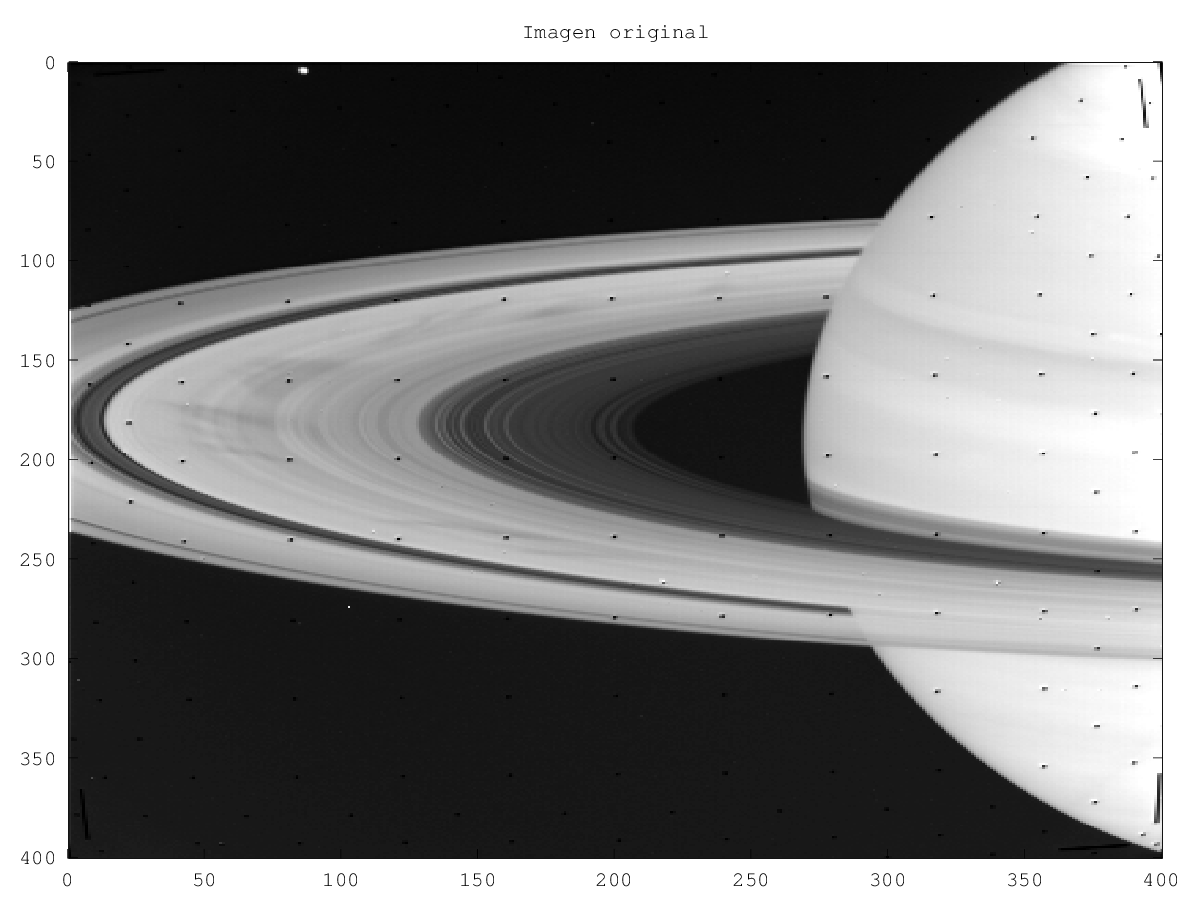
\includegraphics[width=\linewidth]{../images/saturno.png}
        \caption{La imagen original del planeta Saturno.}
        \label{fig:saturno}
\end{figure}

\begin{figure}[H]
        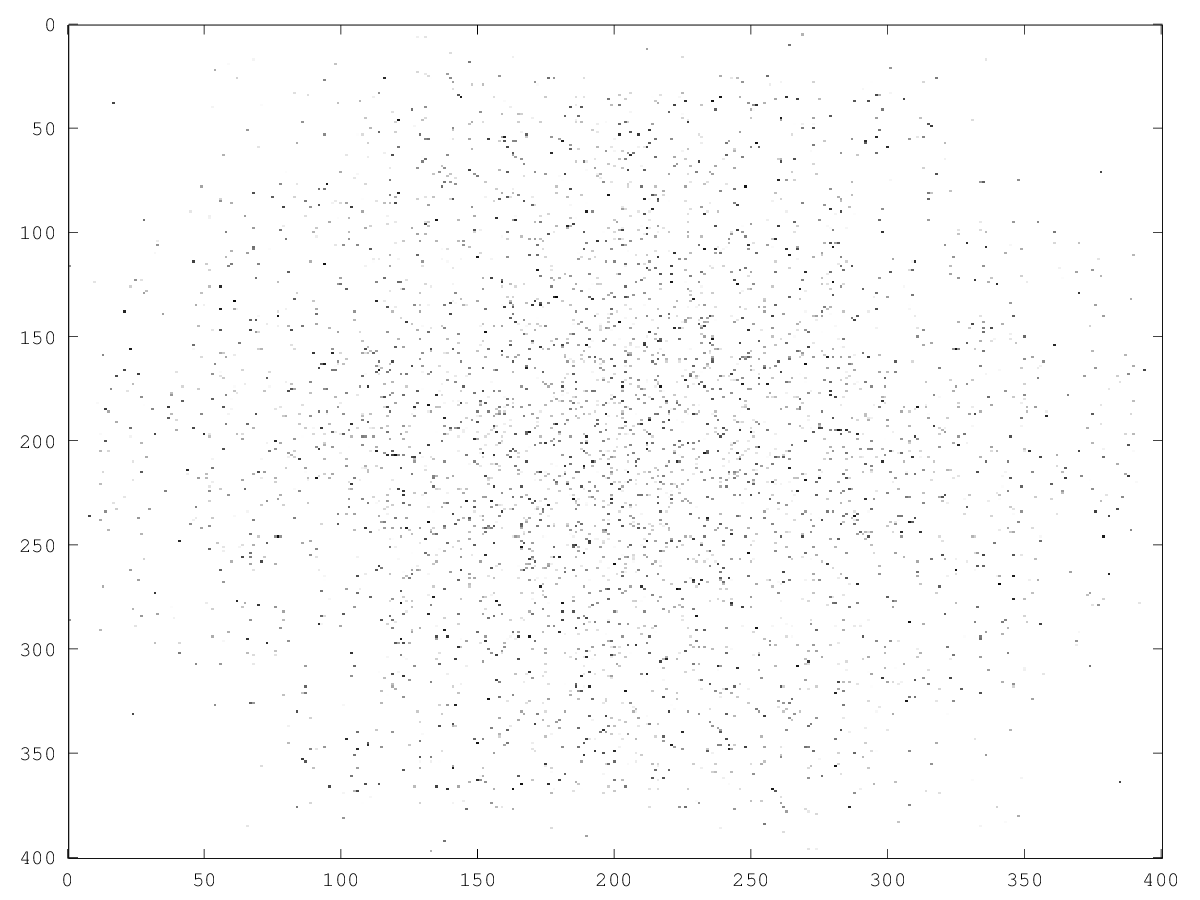
\includegraphics[width=\linewidth]{../images/amplitude.png}
        \caption{La imagen correspondiente a la amplitud. Puede verse como hay una mayor concentraci\'on de puntos alrededor del centro de la imagen, que 
        en las cercan\'ias de los bordes, lo cual indica una mayor cantidad de frecuencias bajas.}
        \label{fig:amplitude}
\end{figure}

\begin{figure}[H]
        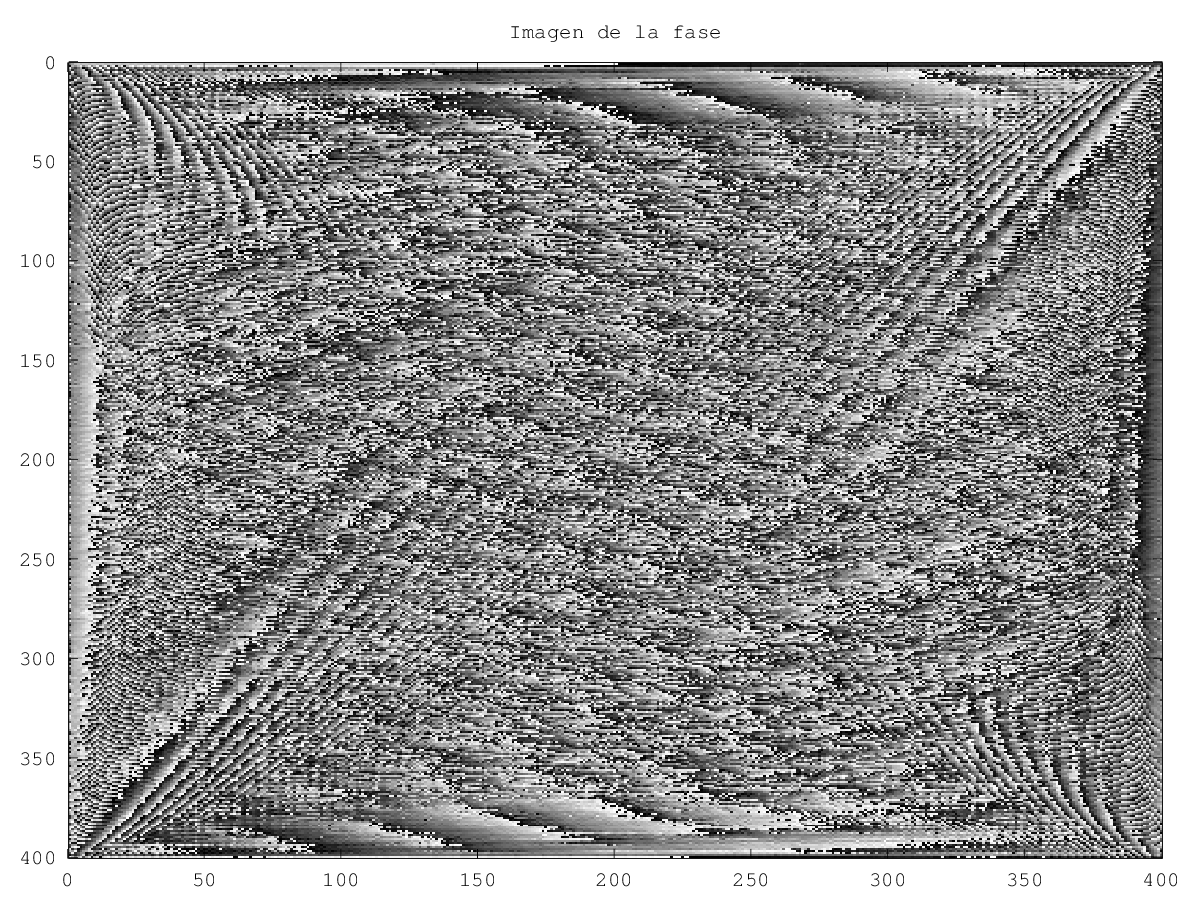
\includegraphics[width=\linewidth]{../images/phase.png}
        \caption{La imagen correspondiente a la fase.}
        \label{fig:phase}
\end{figure}

\begin{figure}[H]
        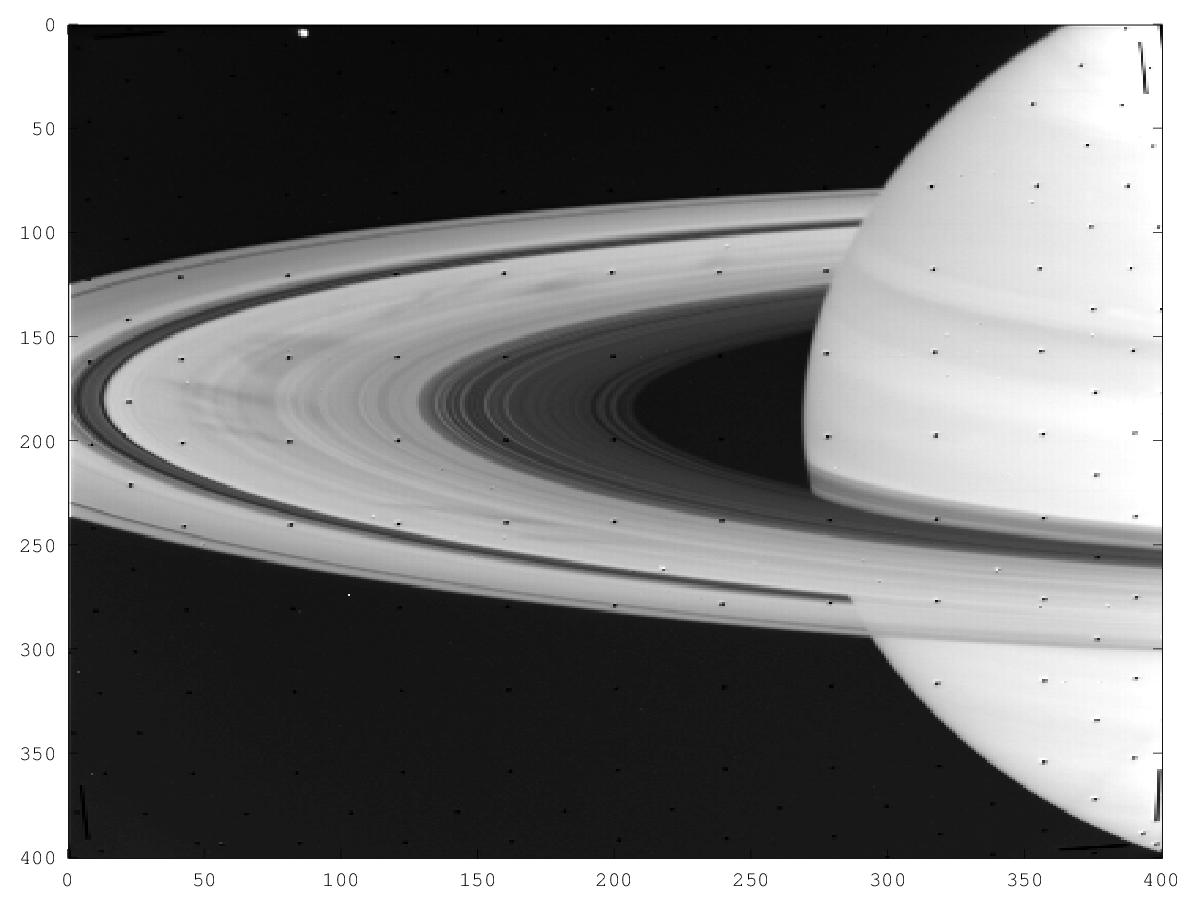
\includegraphics[width=\linewidth]{../images/rebuild.png}
        \caption{La imagen reconstruida luego de transformar y anti-transformar.}
        \label{fig:rebuild}
\end{figure}

\begin{figure}[H]
        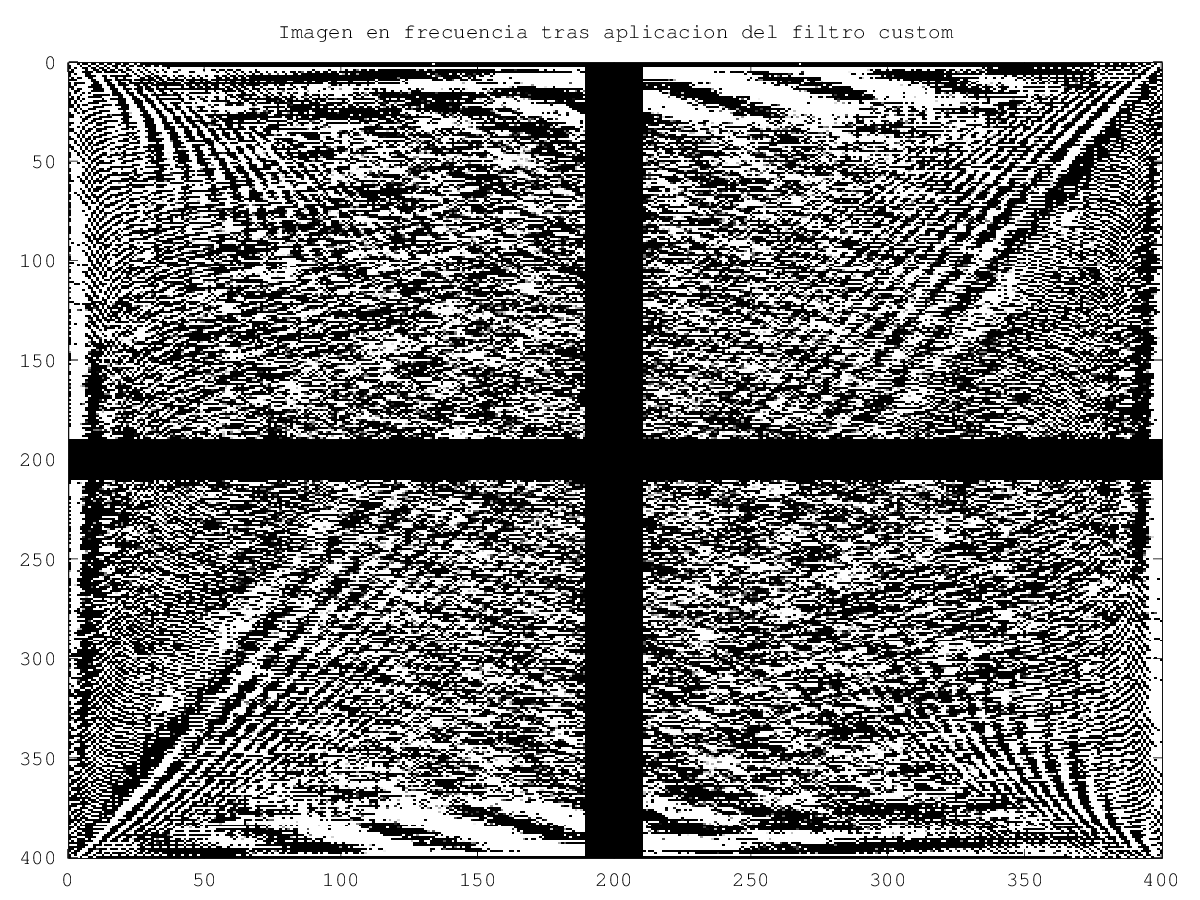
\includegraphics[width=\linewidth]{../images/customFilterFreq.png}
        \caption{La imagen de frecuencias luego de aplicar el filtro custom. Puede verse como se filtran los rangos que el filtro anula.}
        \label{fig:customFilterFrequency}
\end{figure}

\begin{figure}[H]
        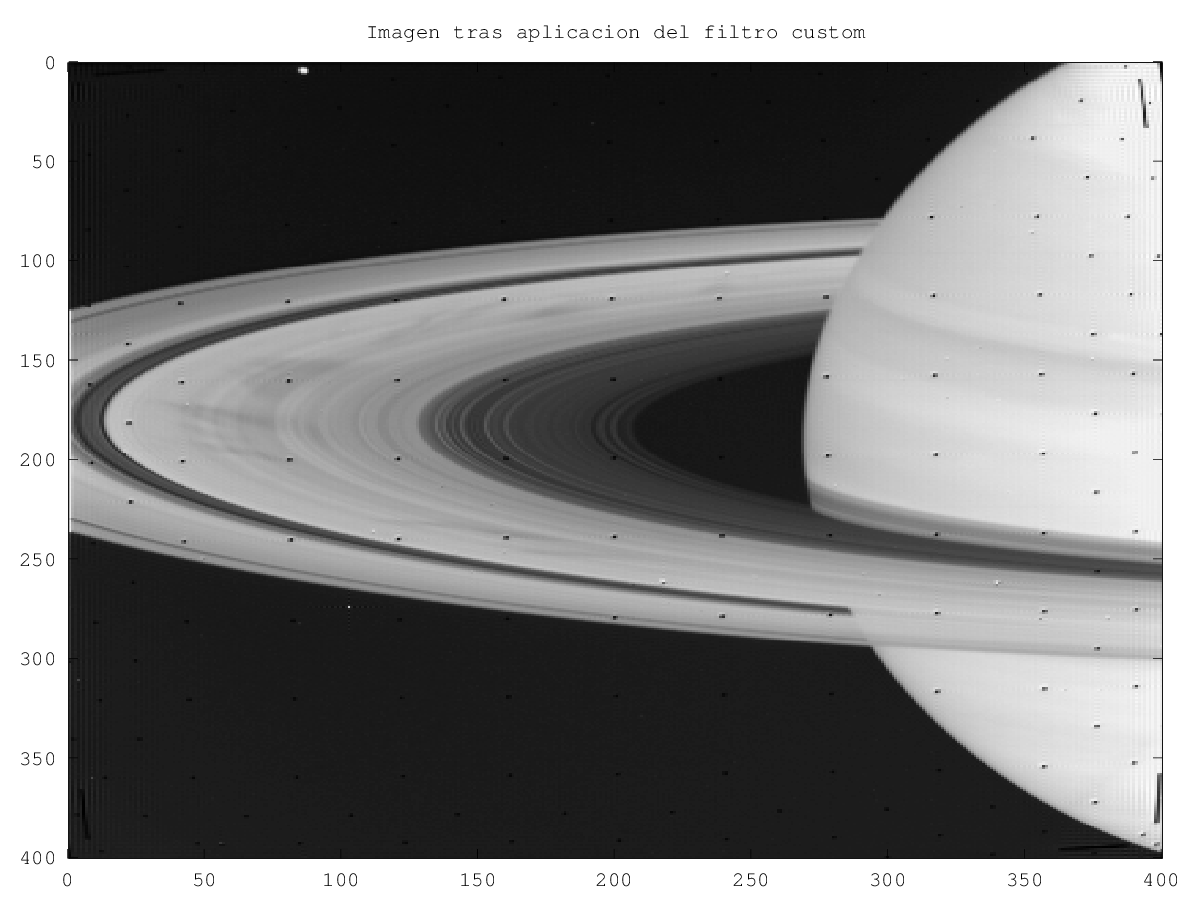
\includegraphics[width=\linewidth]{../images/customFilter.png}
        \caption{La imagen reconstruida luego de la aplicaci\'on del filtro custom. Si se observa bien puede verse como se introduce un poco de ruido 
        en las zonas cercanas a los bordes.}
        \label{fig:customFilter}
\end{figure}

\begin{figure}[H]
        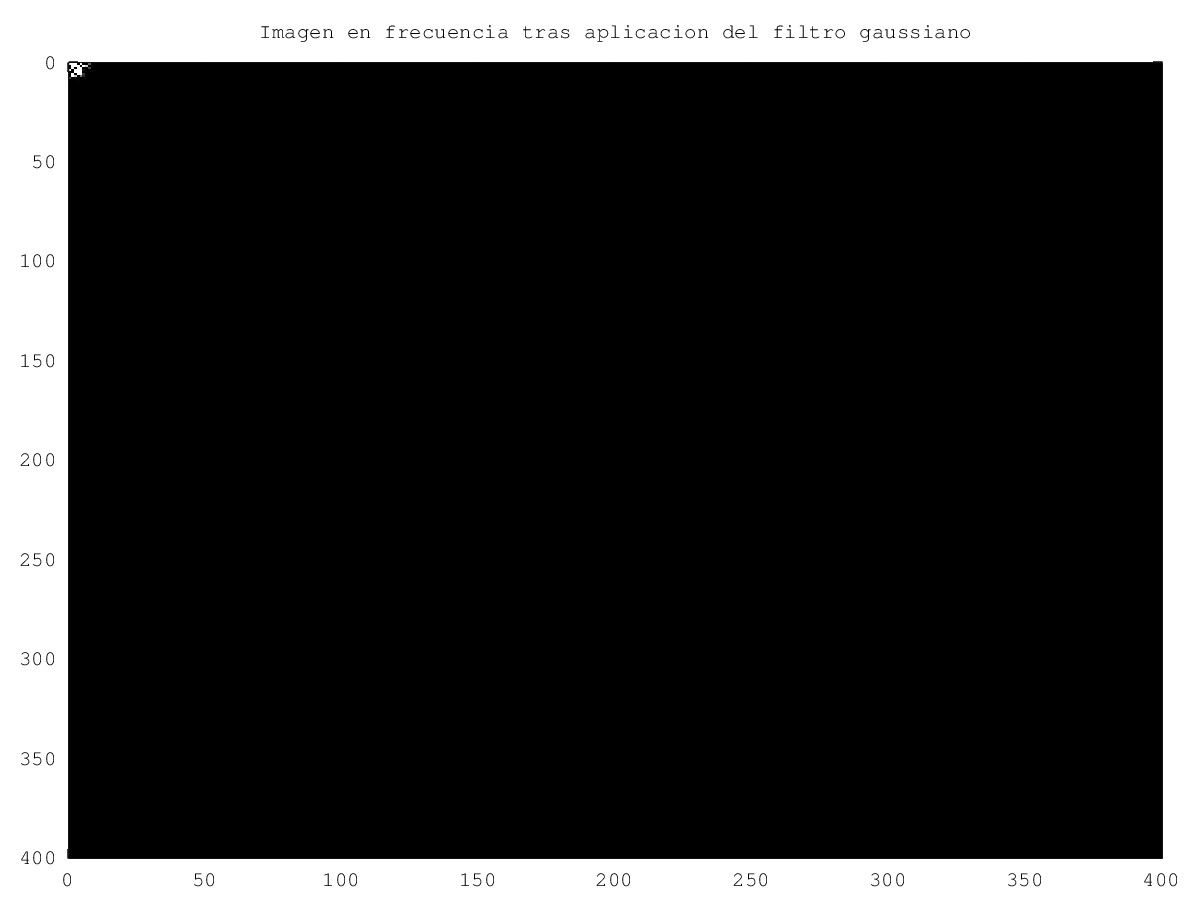
\includegraphics[width=\linewidth]{../images/gaussFilterFreq.png}
        \caption{La imagen de frecuencias luego de aplicar el filtro gaussiano. Es d\'ificil pero puede percibirse que solo las frecuencias muy pequeñas 
        sobreviven, por lo que la imagen es en su gran mayoría de color negro. Este es, entonces, un filtro \textit{pasabajos}.}
        \label{fig:gaussFilterFrequency}
\end{figure}

\begin{figure}[H]
        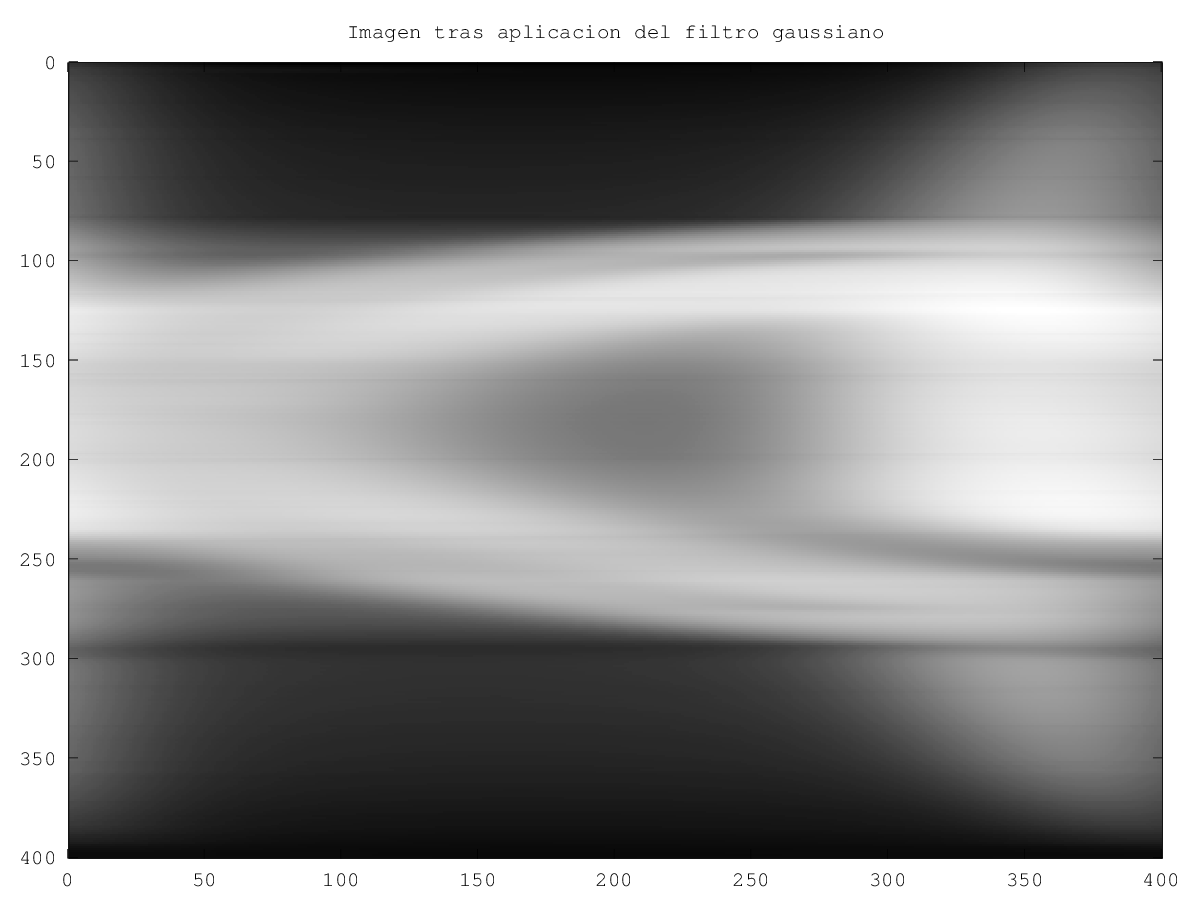
\includegraphics[width=\linewidth]{../images/gaussFilter.png}
        \caption{La imagen reconstruida luego de la aplicaci\'on del filtro gaussiano. Puede verse como este filtro, por ser \textit{pasabajos}, aten\'ua 
        los cambios de colores en la imagen, eliminando los bordes y obteniendo una imagen ``borrosa''.}
        \label{fig:gaussFilter}
\end{figure}

\begin{figure}[H]
        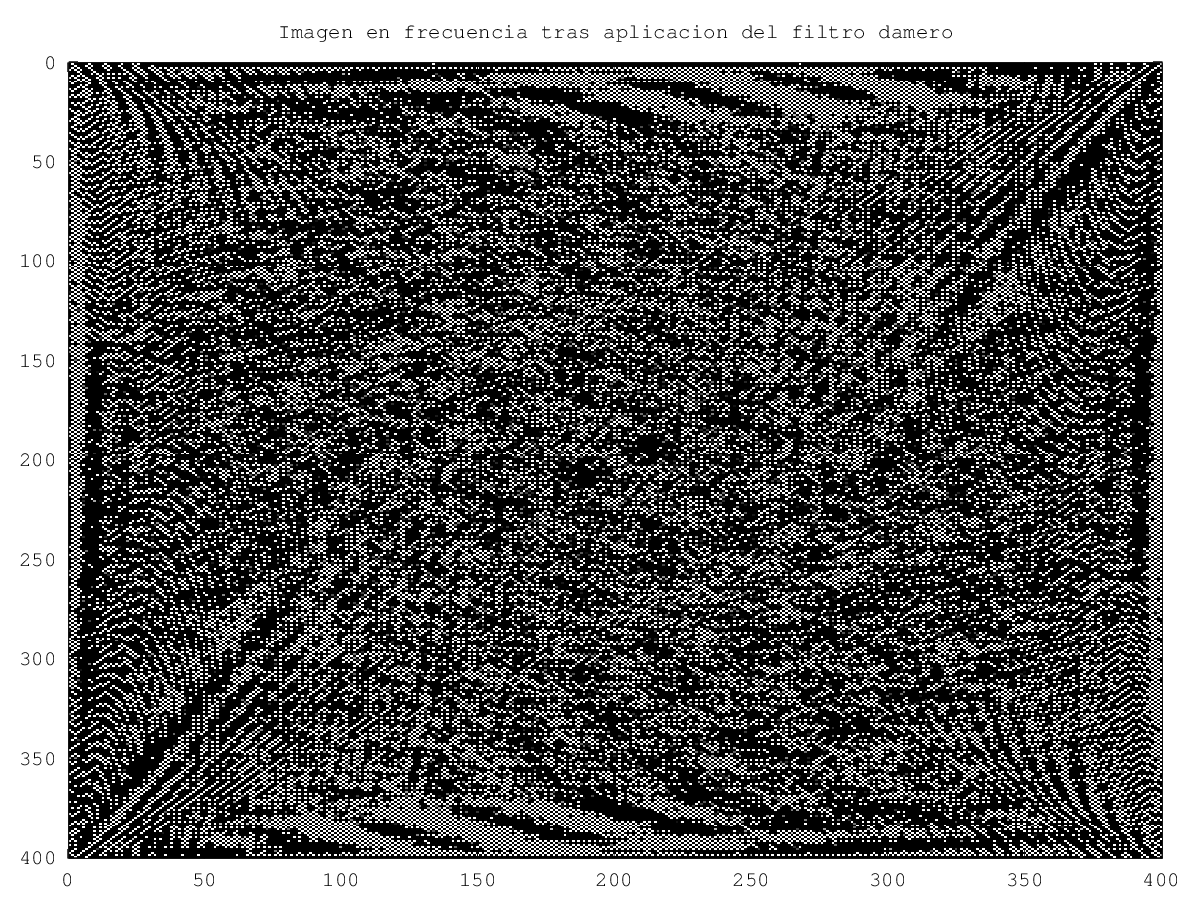
\includegraphics[width=\linewidth]{../images/dameroFilterFreq.png}
        \caption{La imagen de frecuencias luego de aplicar el filtro damero. Es inapreciable ver el efecto del filtro, que filtrando una diagonal y dejando  
        la siguiente, dejando una diagonal como está y la otra en negro, al estilo de una tablero de damas o ajedrez.}
        \label{fig:dameroFilterFrequency}
\end{figure}

\begin{figure}[H]
        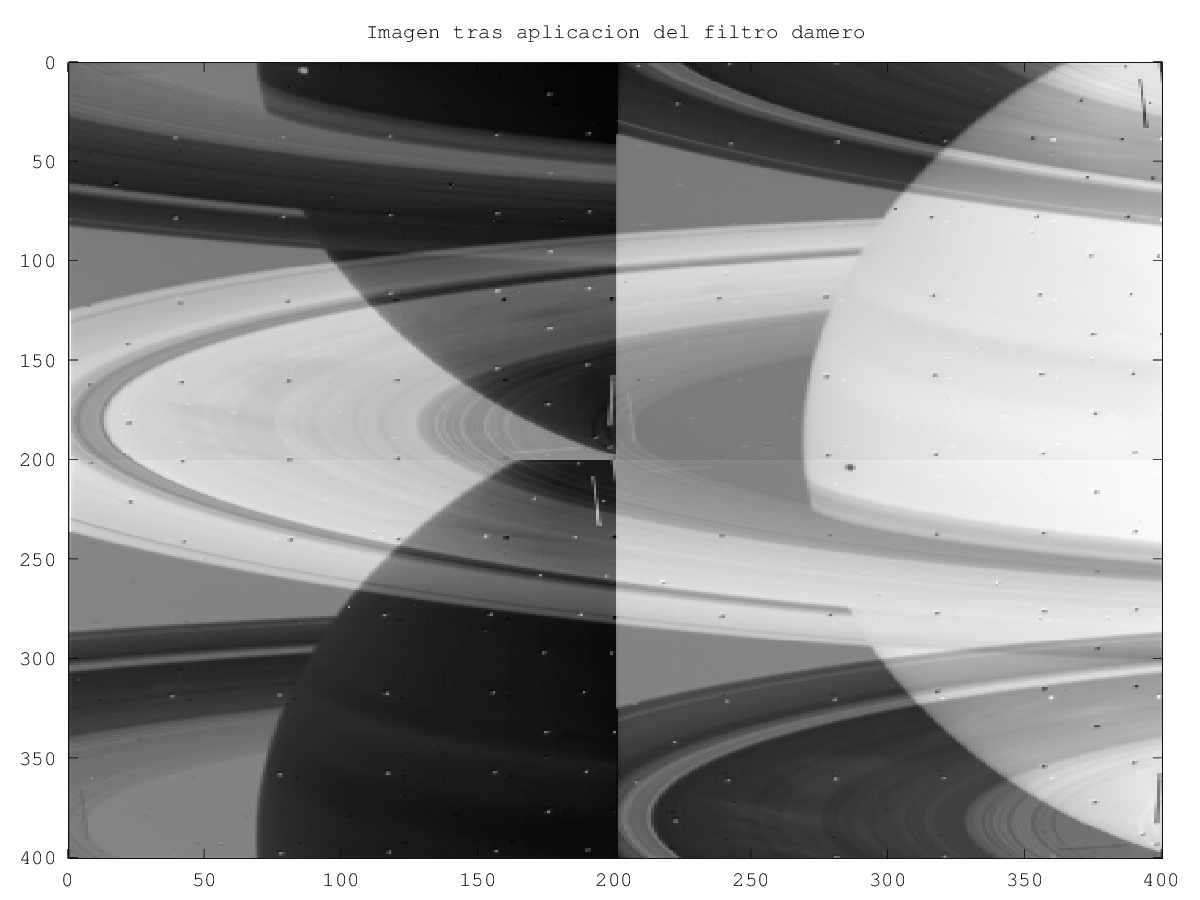
\includegraphics[width=\linewidth]{../images/dameroFilter.png}
        \caption{La imagen reconstruida luego de la aplicaci\'on del filtro damero. El efecto del filtro puede apreciarse a simple vista y resulta muy interesante.
        La imagen ``blanca'' convive con su opuesta, la imagen ``negra'', pero los cuadrantes de esta última se encuentran desordenados.}
        \label{fig:dameroFilter}
\end{figure}

\begin{figure}[H]
        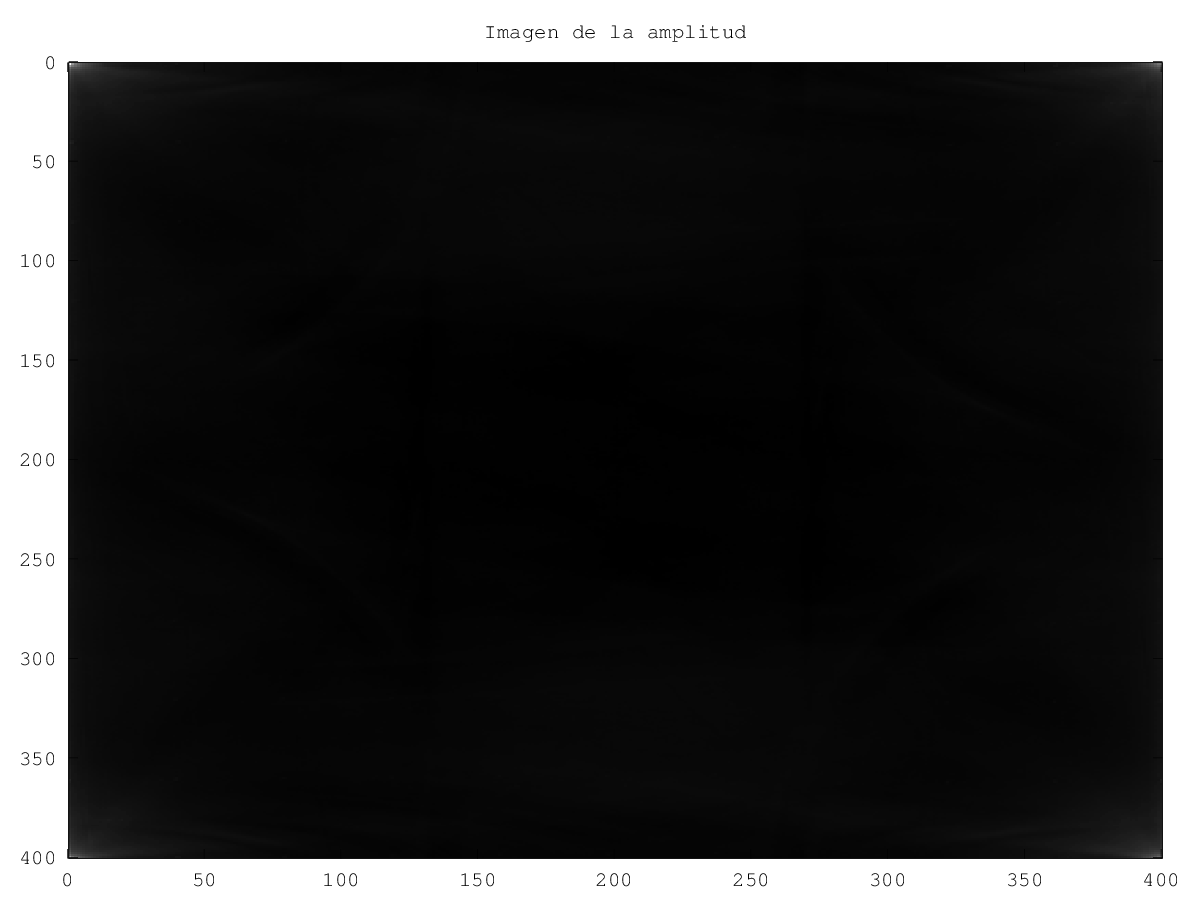
\includegraphics[width=\linewidth]{../images/amplitudeRebuilt.png}
        \caption{La imagen reconstruida a partir de la imagen de la amplitud. Puede observarse que la imagen est\'a totalmente corrupta m\'as all\'a 
        de cualquier tipo de reconocimiento. Esto remarca el hecho de que la informaci\'on de la fase es vital para la reconstrucci\'on de la imagen original.}
        \label{fig:amplitudeRebuilt}
\end{figure}

\end{document}
